\documentclass[12pt, git, final]{rureport}


\begin{document} % this tells the compiler that it is time to make
                 % text to print instead of just getting ready.
\maketitle  % make a title page from the Title, Date, and Author

%\fxnote{skoða titil á skýrslu, sbr. forsíðu}

%\section*{Errata} %%section* avoids putting a number 

\section{Inngangur} % sections break up the document into pieces

Hópverkefni 2 gengur út á það að fara inn á síðuna http://grouplens.org/datasets/movielens/ og ná þar í gagnasett sem inniheldur 10 milljón einkunnargjafir, 100 þúsund 'tags' á 10 þúsund myndum frá 72 þúsund notendum.
\newline
Nemendur eiga svo að skrifa python forrit sem tala við postgresqsl sem geymir MovieLens gagnagrunninn. Forritið á að virka á þann hátt að þegar notandi slær inn heiti á kvikmynd þá á einhvern máta á að birtast notandanum viðbótarupplýsingar þar sem stungið er upp á sambærilegum myndum og myndinni sem var slegin inn í upphafi í forritið.
\section{Framkvæmd}
Byrjað var að taka minna gagnasettið sem inniheldur "aðeins" 100 þúsund einkunnargjafir á 1700 kvikmyndum og unnið með hann í byrjun áður en farið var að ná í stærra gagnasettið.
\begin{itemize} 
	\item Fyrst var náð í minna gagnasettið á http://grouplens.org/datasets/movielens/ sen innheldur 100 þúsund einkunnargjafir á 1700 kvikmyndum og unnið með það til að byrja með.
	\item Við lesum inn 3 skrár og setjum movieId sem index.
	\item Splittum dálkinum upp sem er bæði með ár og titil.
	\item Krill
	\item krill
	\item krill 
	\item krill krill
	\item krillvél
	\item krill maskína
\end{itemize}
 


\section{Niðurstöður}\label{nidurstodur}
\subsection{Hönnun}
Það var ákveðið að hafa GUI og markmiðið var að hafa það einfalt og sem notendavænast því var búinn til sprettigluggi (sjá mynd \ref{fig:cdbf}), sá gluggi hefur 2 dálka, eina leitarstiku og 5 hnappa. Notast var við Qt4 designer til að hanna GUI, það var valið með þeim áherslum að það var auðvelt í notkun og við yrðum hlutfallslega fljótir að hanna GUI útaf þeim stutta tíma sem nemendur höfðu til að skila verkefninu.
\subsection {Virkni}
Eftir að búið er að keyra gui\_test.py skránna þá opnast gluggi og ýtt er á ctrl+E eða ýtt á Database uppi í hægra horninu og þá myndi opnast annar lítill sprettigluggi þar sem viðeigandi upplýsingar eru skráðar inn til að geta tengst gagnagrunninum í gegnum GUI (sjá mynd \ref{fig:dbf2}), ef það er ekki gert þá poppar upp annar sprettigluggi sem lætur notandan vita að hann eigi eftir að slá inn notendaupplýsingu.
\\newline
\\newline
Eftir að búið er að slá inn viðeigandi upplýsingar og þær eru réttar þá birtist annar sprettigluggi sem lætur notendan vita að tenging við gagnagrunn hafi tekist, ef upplýsingarnar eru rangar þá kemur sprettiglugginn með upplýsingar að tenging hafi ekki tekist.
\newline
\newline
Þegar notandinn er búinn nær að tengjast gagnagrunninum þá getur hann skrifað þá mynd sem hann leitar eftir í leitarstikuna og ýtir svo á search, niðurstöðurnar birtast svo í vinstri dálknum ef notendanum líst svo á einhverja mynd sem koma upp við leitina  getur hann bætt henni við á listan yfir myndir sem hann vill velja, með því að ýta á á 'add' hnappinn og þá dettur myndin í vinstri dálkinn (sjá mynd \ref{fig:dbf6}), þegar ýtt er á 'done' hnappinn þá poppar upp annar spretti gluggi sem kemur með myndir sem þér líkar við (sjá mynd \ref{fig:dbf10}), eftir það er hægt að prófa aðrar myndir með því að ýta á 'yes' hnappinn annar ýtir notandinn á 'no' hnappinn og þá ferðu út úr GUI.

\pagebreak
\begin{figure}
	\centering 
	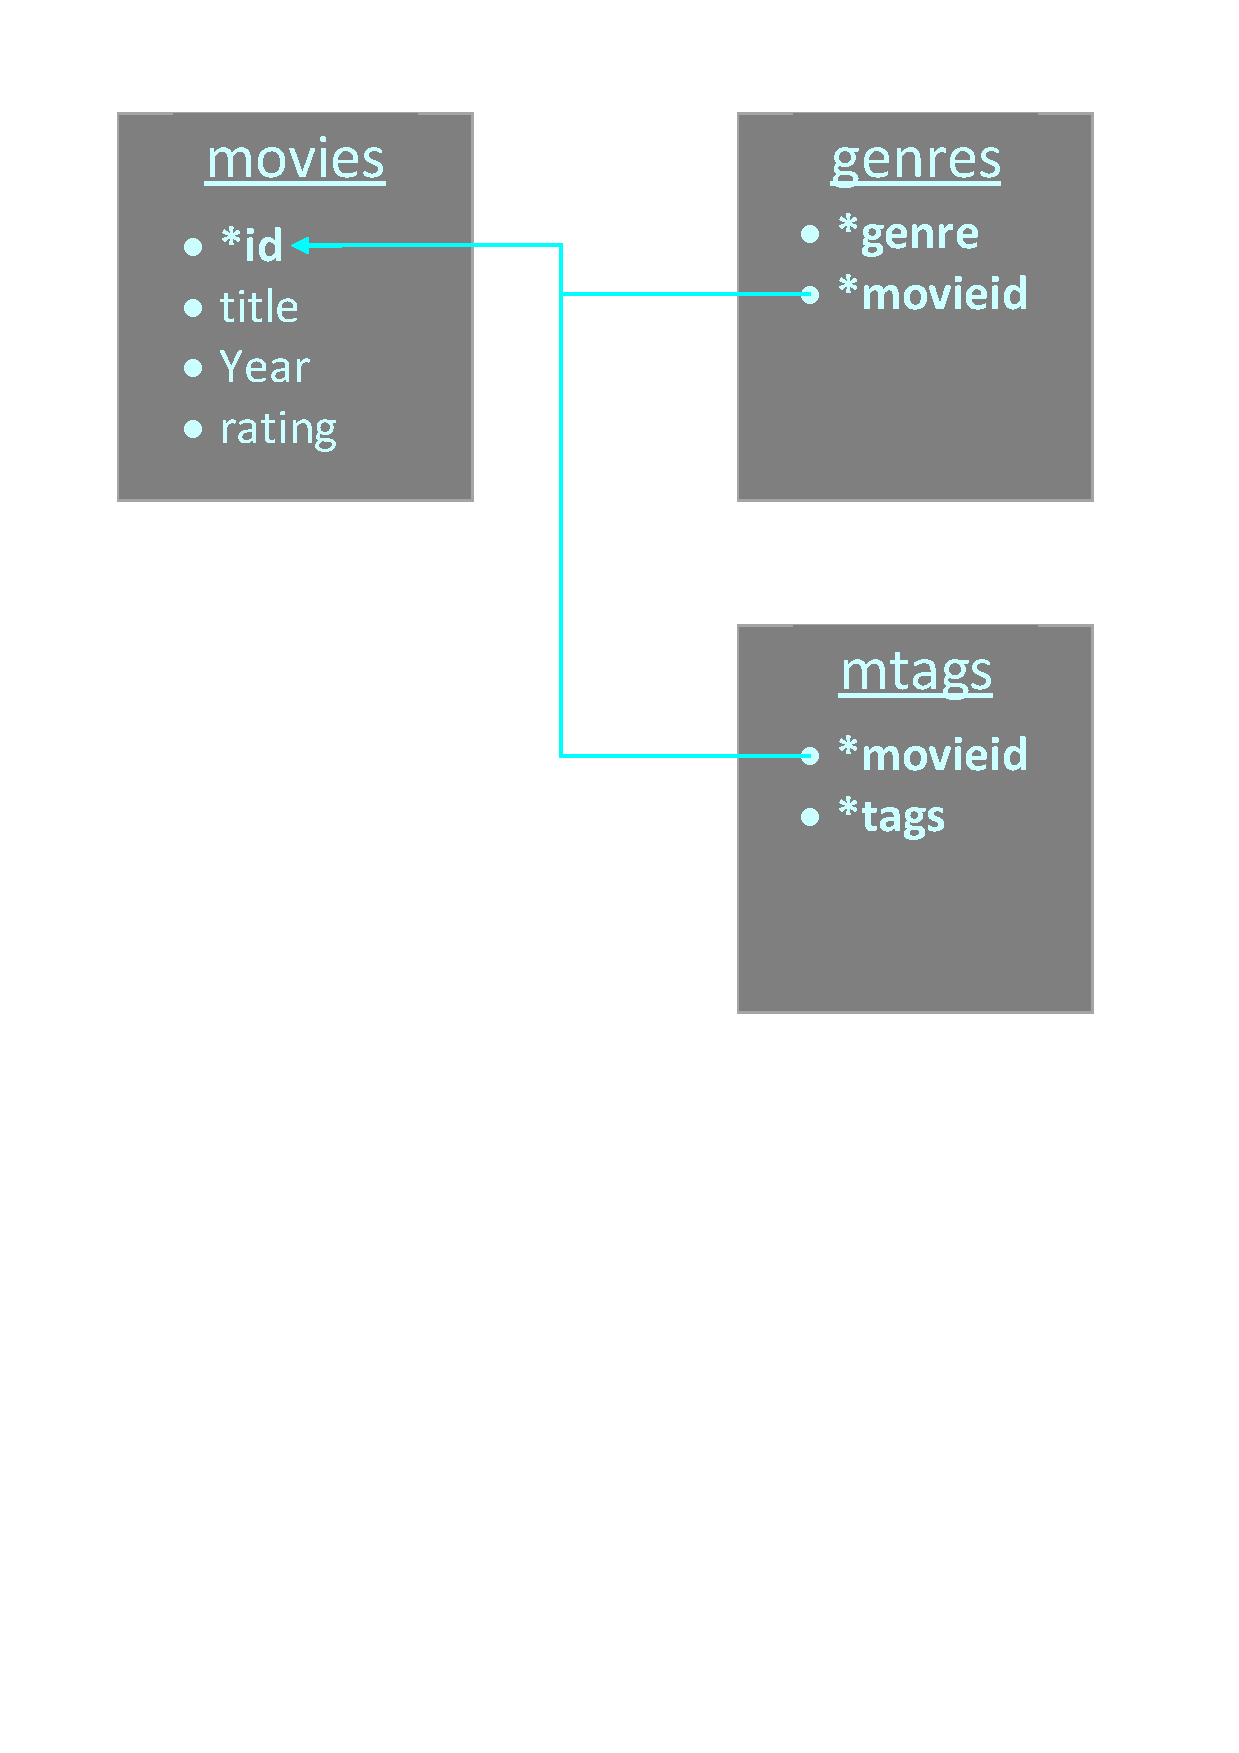
\includegraphics[width=\textwidth]{../graphics/ds.pdf}
	\caption{Database schema \label{fig:dataschema}}
\end{figure}

\begin{figure}
	\centering 
	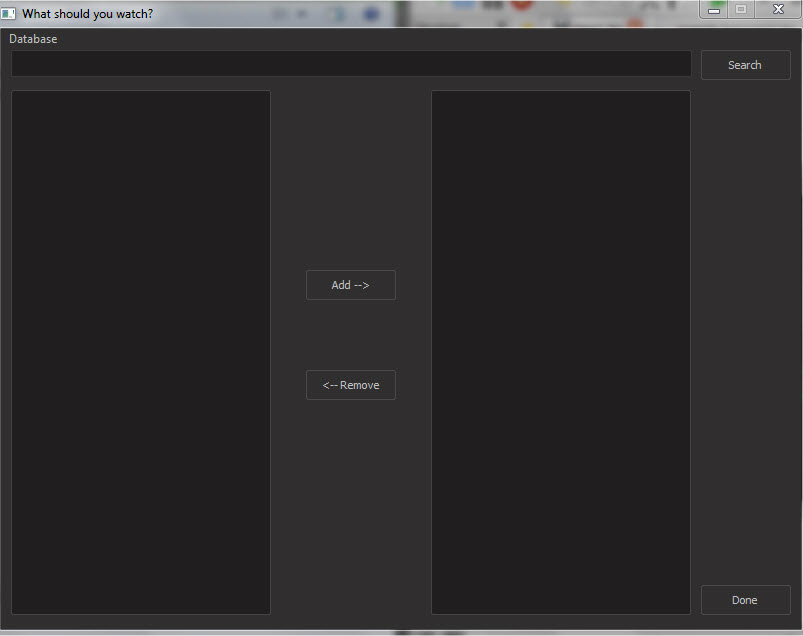
\includegraphics[width=\textwidth]{../graphics/cdbf.png}
	\caption{Sprettigluggi \label{fig:cdbf}}
\end{figure}

\begin{figure}
	\centering 
	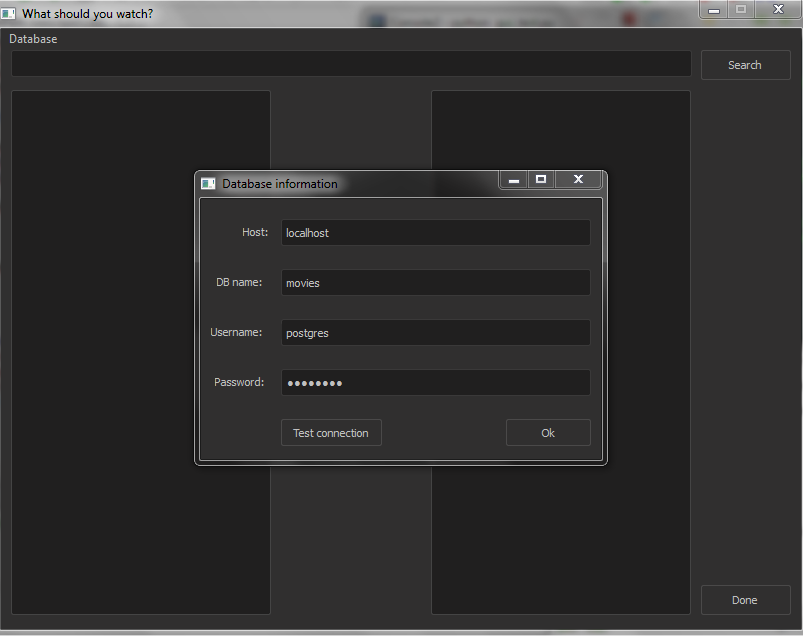
\includegraphics[width=\textwidth]{../graphics/dbf2.png}
	\caption{Sprettiglugginn með upplýsingum útfylltum \label{fig:dbf2}}
\end{figure}


\begin{figure}
	\centering 
	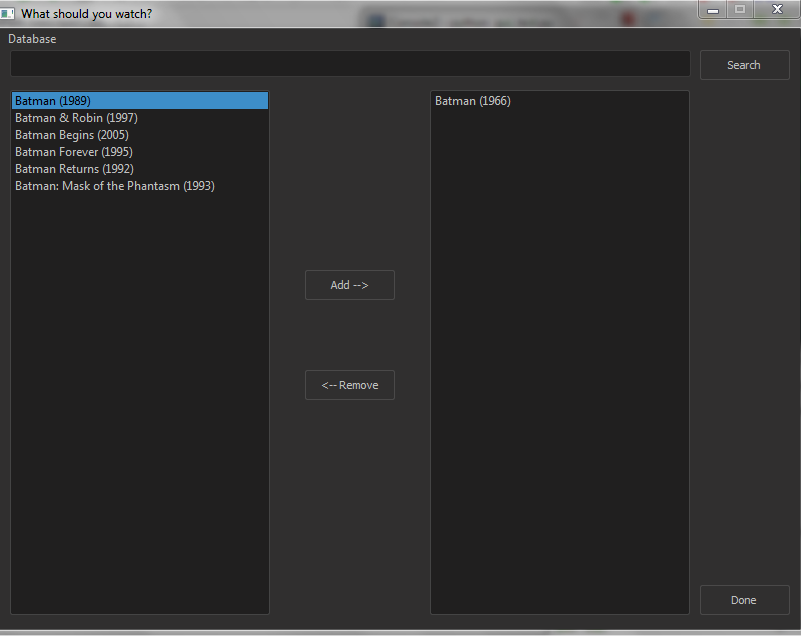
\includegraphics[width=\textwidth]{../graphics/dbf6.png}
	\caption{Niðurstöðrnar úr leitinni\label{fig:dbf6}}
\end{figure}

\begin{figure}
	\centering 
	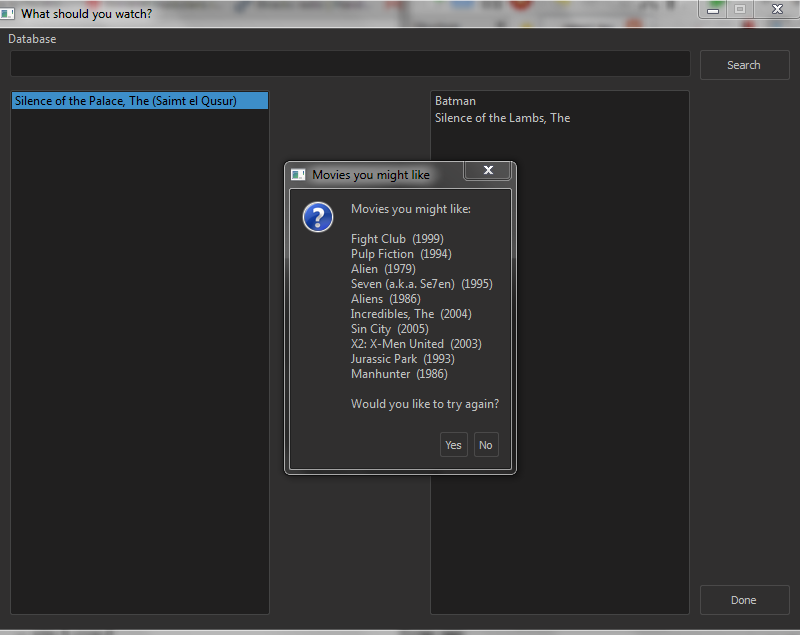
\includegraphics[width=\textwidth]{../graphics/dbf10.png}
	\caption{Niðurstöðrnar úr leitinni\label{fig:dbf10}}
\end{figure}

\clearpage
\printbibliography

\end{document} % this tells the compiler that we are done

% These are variables for the editor Emacs
%%% Local Variables: 
%%% TeX-command-BibTeX: biber
%%% mode: latex
%%% TeX-master: t
%%% End:
